\documentclass{article}
\usepackage[a4paper,]{geometry}
\usepackage{lmodern}
%\usepackage[export]{adjustbox}
\usepackage[utf8]{inputenc}
\usepackage[T1]{fontenc}
\usepackage{graphicx}
%\usepackage{titlepic}
\usepackage{mathtools}
%\usepackage{amsmath}
%\usepackage{amssymb}
%\usepackage{amsfonts}
%\usepackage{accents}
%\usepackage{esvect}
%\usepackage{subcaption}
\usepackage{multicol}
\usepackage{hyperref}
%\usepackage{enumitem}
\usepackage[makeroom]{cancel}
\usepackage{siunitx}
\usepackage{float}
\usepackage{lipsum}
\usepackage{textcomp}

\sisetup{separate-uncertainty=true}
\linespread{1.3}

% my commands
\newcommand{\E}[1]{\, \mathrm{e}{#1} \, }
\newcommand{\de}{\mathrm{d}}
\newcommand{\pars}{\mathbin{\!/\mkern-5mu/\!}}
\newcommand{\equalexpl}[1]{
	\underset{\substack{\uparrow\\\mathrlap{\text{#1}}}}{=}}


\title{Misure Resistenza}
\author{Filippo Dal Farra \and Matteo Zandegiacomo Orsolina}
\date{19 Novembre 2018}

\begin{document}

\maketitle

\newpage

\section{Introduzione}

Questa relazione riassume gli esiti di tre esperienze tutte finalizzate all'adempimento dell'analisi di un circuito RLC svolto durante l'ultima seduta. Per fare ci\'o si \'e sfruttato l'uso di un oscilloscopio il quale, da come si vedr\'a, modifica inevitabilmente le risposte dei circuiti in analisi. A causa di questo è risultato poi necessario derivare i valori delle capacità e delle resistenze parassite che si trovano all'interno dell'oscilloscopio per poi effettuare l'analisi tenendo conto di esse. \\

Successivamente abbiamo studiato la risposta in frequenza del circuito RC nelle diverse configurazioni di filtro passa alto e filtro passa basso, sempre variando le frequenze di taglio. Così facendo si \'e riusciti ad ottenere i diagrammi di Bode corrispondenti che associati alle funzioni di trasferimento teoriche associate forniscono i valori dei componenti usati nei vari casi. Inoltre queste misure sono poi state messe a confronto con i risultati ottenuti precedentemente nella carica e scarica del condensatore, per osservare se queste misure erano tra loro compatibili. \\

Infine abbiamo considerato anche un induttore, consistente in una bobina realizzata precedentemente. Inizialmente abbiamo studiato un circuito RL per trovate il valore dell'induttanza di questo elemento attraverso diversi cicli di carica e scarica del campo magnetico da esso generato. In seguito è stata posta all'interno di un circuito RLC composto dalla bobina e dal condensatore usato precedentemente di cui si sapeva a questo punto il valore. Ciò ci ha permesso di studiare il funzionamento del circuito passa banda e la propria frequenza di risonanza.

\newpage

\section{Materiali e strumenti}

\begin{itemize}
  \item Svariate resistenze da usare a seconda delle necessità
  \item Un condensatore
  \item Cavi "banana-banana"
  \item Breadboard
  \item Bobina precedentemente realizzata
  \item Multimetro digitale (DMM)
  \item Generatore di tensione variabile
  \item Oscilloscopio
  \item %TODO: Non mi viene in mente altro, ma di sicuro ho dimenticato qualcosa
\end{itemize}

\newpage

\section{Procedure di misura}

Innanzitutto è stato necessario montare il circuito RC per osservare la scarica del condensatore come suggerito dalla scheda fornita \ref{fig:RC_LP}. Ad esso andava poi collegato l'oscilloscopio tramite i cavi coassiali all'ingresso ed all'uscita del circuito. Abbiamo noi impostato il generatore di funzioni in modo che  producesse lo scalino da $\Delta V$ a $0\ V$ , e in questa configurazione \'e stato osservato l'andamento in uscita dell'onda nella fase di scarica. Sono stati utilizzati 5 diversi valori di resistenza con lo stesso condensatore in modo da avere tempi caratteristici $\tau$ differenti e per ognuno sono state salvate 6 forme d'onda con l'oscilloscopio impostato a 16 averagings. Ciò ha fornito un numero sufficiente di dati per poi poter trovare i parametri relativi ad eventuali componenti parassiti dato che la procedura \'e stata ripetuta senza il condensatore in esame supplito dalla capacit\'a intrinseca in cavi e ADC dell'oscilloscopio. Tutti i valori di resistenza utilizzati sono stati misurati con il DMM. \\

Successivamente lo stesso circuito \'e stato da noi studiato come filtro, analizzando la sua risposta ad un ingresso sinusoidale in funzione della frequenza applicata. Sono stati da noi scelti valori di resistenza che ci dessero valori della frequenza di taglio specifici, il generatore di funzioni \'e stato impostato da noi a $V_{PP} = 2 \ V$ %TODO:check vpp
con frequenze distribuite esponenzialmente per una decade e \textonehalf \ prima e dopo la frequenza di taglio. Quindi sono stati da noi trascritti i valori di ampiezza in entrata ed uscita dal circuito assieme allo sfasamento tra i due forniti dall'oscilloscopio tramite le sue funzioni di misura in modo da poter creare il diagramma di Bode. Infine abbiamo noi applicato una resistenza in modo da caricare il circuito ed in queste condizioni \'e stata misurata l'impedenza in uscita del filtro con due diverse frequenze. La procedura è stato ripetuta con la configurazione passa alto \ref{fig:RC_HP}, per un unico valore di resistenza. \\


% TODO: devo ancora leggere
In seguito si è considerata una bobina costruita precedentemente e con essa è stato costruito un circuito RL. Per fare ciò la bobina è stata inserita all'interno di una struttura fatta da un materiale ferromagnetico, il quale aveva come ruolo quello di ampliare l'induttanza da esso prodotta. Si è innanzitutto ancora usata un'onda quadra dal generatore di funzioni, con diverse configurazioni di resistenze. Se ne è così studiata la carica e la scarica di questo elemento. Si è poi montato un circuito RLC passa banda, sfruttando come induttore ancora la bobina e come condensatore l'elemento di circuito usato precedentemente. Si è impostato il generatore di funzioni in modo da realizzare un'onda sinusoidale applicata a due diverse configurazioni di valori di resistenza. Si è studiato ciò modificando i valori della frequenza, e la maggior parte di essi sono stati presi in concomitanza della frequenza di risonanza del circuito.

\newpage

%%%%%%%%%%%%% ANAL-isis %%%%%%%%%%%%%%%%%%%

\section{Analisi dei dati}

Verranno ora analizzati i dati ottenuti per ogni configurazione.

\subsection{Scarica condensatore}

Il circuito ora preso in considerazione \'e il seguente:

\begin{figure}[h]
    \centering
    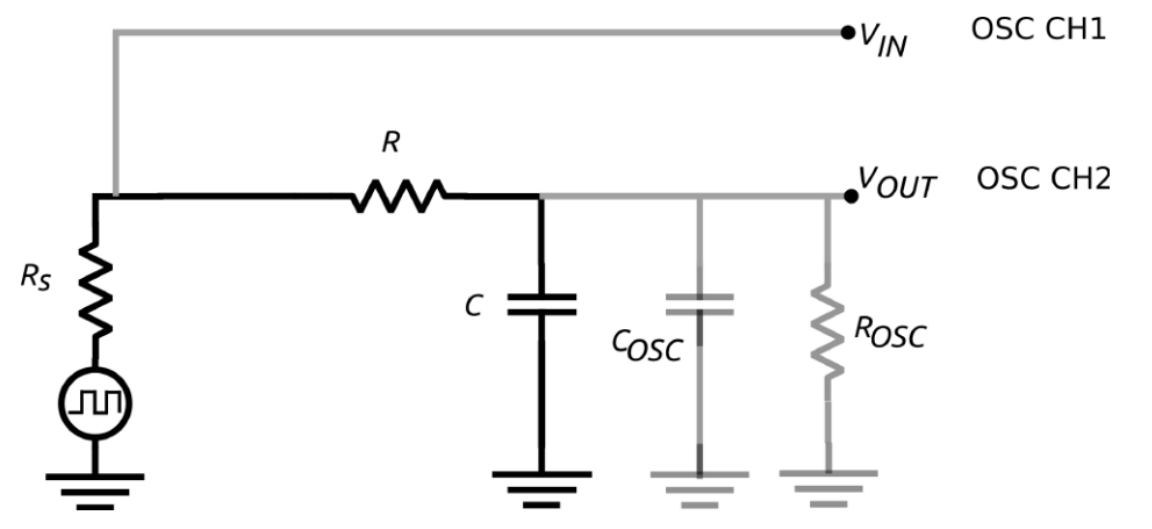
\includegraphics[width = \textwidth]{RC_LP.png}
    \caption{Circuito RC passa basso utilizzato anche per l'analisi della scarica del condensatore}
    \label{fig:RC_LP}
\end{figure}

Utilizzando la legge di Kirchhoff per le tensioni e presa la maglia passante per la resistenza $R$ e condensatore $C$ e considerando la relazione tra corrente e tensione ai capi di esso \ref{eq:cap_law} si ottiene l'equazione differenziale \ref{eq:cap_equ} che rappresenta una semplificazione di quello che accade nel nostro circuito nell'approssimazione $C_{osc}=0$ e $R_{osc} = \infty $.

\begin{gather}
    i(t) = C \frac{\de V_c (t)}{\de t}
    \label{eq:cap_law} \\   
    \nonumber V_{in} - i(t) R - V_c(t) = 0 \Rightarrow \\
    \tau \frac{\de V_c(t)}{\de t} + V_c(t) = V_{in} \quad \textrm{con} \quad \tau = RC
    \label{eq:cap_equ}
\end{gather}

Date le condizioni iniziali di condensatore carico a $V_c(t = 0) = \Delta V$ che \'e il livello di tensione alta del generatore di funzioni il quale per $t > 0$ fornisce $V_{in} = 0$ si ottiene la forma analitica della scarica del condensatore \ref{eq:cap_dis} risolvendo l'equazione differenziale corrispondente.

\begin{gather}
	\nonumber 
	\frac{\de V_c(t)}{\de t} = - \frac{1}{\tau} V_c(t) \\
	V_c(t) = \Delta V \exp{- \frac{t}{\tau}}
	\label{eq:cap_dis}
\end{gather}

Tuttavia l'applicazione del circuito di misura, l'oscilloscopio nel nostro caso, e la presenza della resistenza in uscita del generatore provocano inevitabilmente una modifica del caso ideale, in particolare $R_{osc}$ fa un partitore di tensione con $R$ e $R_{s}$ cos\'i che il condensatore non \'e inizialmente carico alla tensione del generatore e la sua scarica avviene anche attraverso $R_{osc}$.
L'equazione \ref{eq:cap_dis} si sostituisce quindi con l'equazione \ref{eq:cap_dis_real} che tiene conto dei componenti parassiti.

\begin{gather}
	\nonumber 
	V_0 = \Delta V \frac{R_{osc}}{R_{osc} + R + R_{s}} \\ 
	\tau = ( C_{osc} + C ) ( (R + R_s) \pars R_{osc} ) \\
	V_{out}(t) = V_c(t) = V_0 \exp{ -\frac{t}{\tau} }
	\label{eq:cap_dis_real}
\end{gather}

A scopo rappresentativo viene quindi mostrata una delle forme campionate:

\begin{figure}[h]
    \centering
    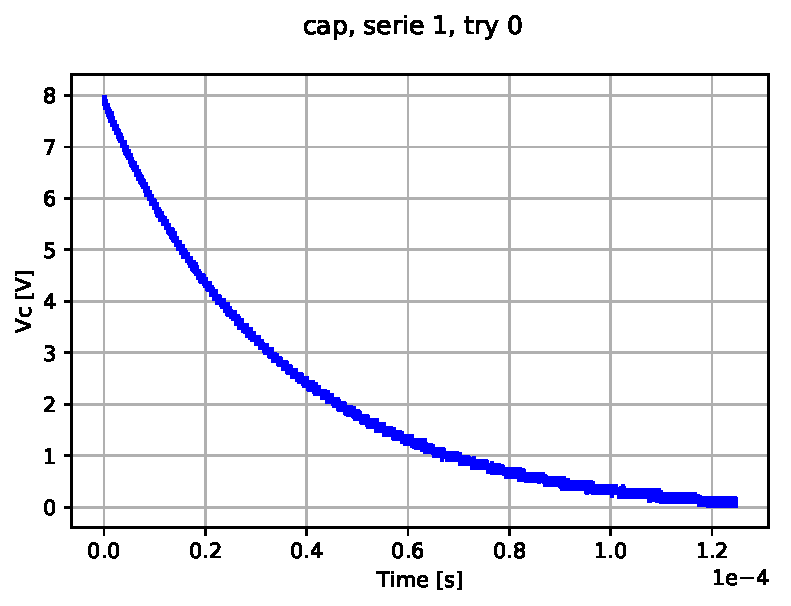
\includegraphics[width = 0.5\textwidth]{capserie1try0.pdf}
    \caption{Primo campione preso con il primo valore di resistenza, si nota qualitativamente che la scarica \'e compatibile con una caduta esponenziale}
    \label{fig:cap_dis_ex}
\end{figure}

La relazione \ref{eq:cap_dis_real} che rappresenta la scarica del condensatore in funzione del tempo pu\'o essere linearizzata in questa variabile se viene preso il logaritmo di $V_{out}$ \ref{eq:cap_dis_lin}.

\begin{gather}
	\ln{V_{out}(t)} = \ln{ \left( V_0 \exp{ -\frac{t}{\tau} } \right) } = \ln{V_0} + \left( -\frac{1}{\tau} \right) t = A + B t \\
	\sigma[\ln{V_{out}}]=\frac{\sigma[V_{out}]}{V_{out}}
	\label{eq:cap_dis_lin}
\end{gather}

\begin{figure}[h]
    \centering
    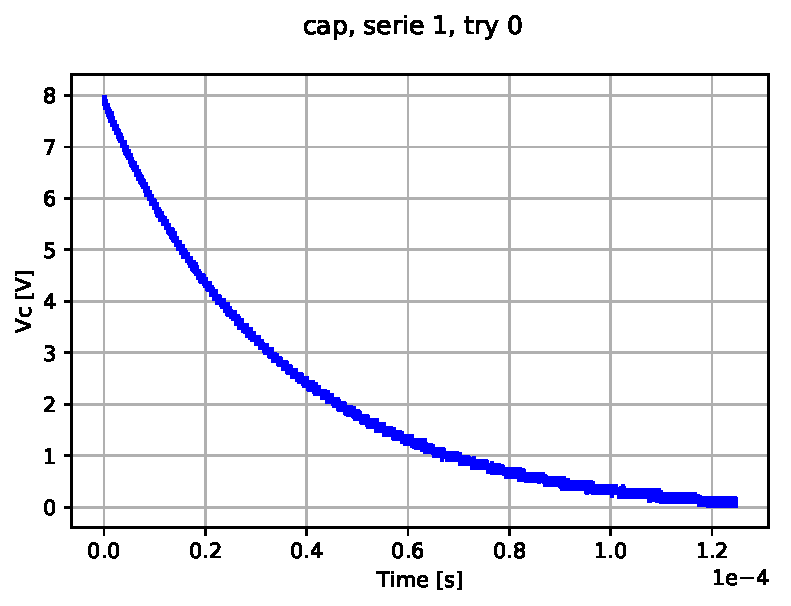
\includegraphics[width = 0.5\textwidth]{capserie1try0.pdf}
    \caption{Fit lineare della scarica del condensatore}
    \label{fig:cap_dis_ex_lin}
\end{figure}

Si pu\'o quindi procedere al fit lineare per il calcolo dei parametri $A$ e $B$ e il rusultato con il confronto tra modello e campioni \'e mostrato in figura \ref{fig:cap_dis_ex_lin}. Come si pu\'o vedere, avvicinandosi a $V_c = 0$ i campioni presi mostrano un drift dal modello: questo \'e molto probabilmente dovuto ad un offset sullo zero dell'oscilloscopio e tale ipotesi viene quindi ora analizzata.

La presenza di un offset $\delta V$, assunto fisso, in fase di misura non ci permette di applicare la regressione lineare del caso precedente: 

\begin{gather}
	\nonumber
	V_m(t) = V_{out}(t) + \delta V =  V_0 \exp{ -\frac{t}{\tau} } + \delta V
	\\
	\nonumber
	\ln{V_m(t)} \equalexpl{\hspace{-2.5em}$V_{out} \approx V_m$} 
	\ln{\left( V_0 \exp{ -\frac{t}{\tau} } \right) } + 
	\ln{\left( 1 + \frac {\delta V}{V_{m}} \right) } = 
	\\
	\nonumber
	\equalexpl{\hspace{-4.5em}$\ln(1+x) = x + o(x)$} 
	\ln{\left( V_0 \exp{ -\frac{t}{\tau} } \right) } + 
	\frac {\delta V}{V_m} = A + B t + C\frac{1}{V_m}
	\\
	A = \ln{V_0} \quad B = -\frac{1}{\tau} \quad C = \delta V
	\label{eq:gen_reg}
\end{gather}  

Si procede quindi ad applicare la regressione generalizzata \ref{eq:gen_reg} ed i risultati per ogni serie di dati presa in considerazione sono rappresentati nelle tabelle \ref{eq:gen_reg}.


















\begin{figure}[h]
\begin{center}
    \large{Amperometro a monte}
\end{center}
\begin{multicols}{2}
\begin{center}
\begin{tabular}{c|c} 
$V_{FS}=\SI{10}{\volt}$&$i_{FS}=\SI{5}{\milli\ampere}$\\
$V_i \pm \sigma [V]$ [\si{\volt}] & $i_i \pm \sigma [i]$ [\si{\milli\ampere}]\\
[0.5ex]
\hline
$9.6 \pm 0.2 $&$2.2 \pm 0.1$\\

$7.8 \pm 0.2 $&$1.7 \pm 0.1$\\

$8.6 \pm 0.2 $&$1.9 \pm 0.1$\\

$8.6 \pm 0.2 $&$1.8 \pm 0.1$\\

$7.2 \pm 0.2 $&$1.5 \pm 0.1$\\

$7.2 \pm 0.2 $&$1.6 \pm 0.1$\\

$5.6 \pm 0.2 $&$1.2 \pm 0.1$\\

$6.0 \pm 0.2 $&$1.3 \pm 0.1$\\

$8.0 \pm 0.2 $&$1.7 \pm 0.1$\\

$8.8 \pm 0.2 $&$1.9 \pm 0.1$\\

\end{tabular}
\end{center}

\begin{center}
\begin{tabular}{c|c} 
$V_{FS}=\SI{2}{\volt}$&$i_{FS}=\SI{500}{\micro\ampere}$\\
$V_i \pm \sigma [V]$        [\si{\volt}] & $i_i \pm \sigma [i]$         [\si{\milli\ampere}]\\
[0.5ex]
\hline
$1.80 \pm 0.04 $& $0.43 \pm 0.01$\\
$1.36 \pm 0.04 $&$0.33 \pm 0.01$\\

$1.40 \pm 0.04 $&$0.34 \pm 0.01$\\

$1.64 \pm 0.04 $&$0.39 \pm 0.01$\\

$1.52 \pm 0.04 $&$0.37 \pm 0.01$\\

$1.56 \pm 0.04 $&$0.38 \pm 0.01$\\

$1.20 \pm 0.04 $&$0.29 \pm 0.01$\\

$1.92 \pm 0.04 $&$0.46 \pm 0.01$\\

$1.76 \pm 0.04 $&$0.43 \pm 0.01$\\

$1.68 \pm 0.04 $&$0.40 \pm 0.01$\\

\end{tabular}
\end{center} 
\end{multicols}
\end{figure}

\newpage

\section{Conclusioni}
\lipsum[1-2]
Non funziona un cazzo
\end{document}
